% Created 2012-12-17 Mon 03:07
\documentclass[11pt]{article}
\usepackage[utf8]{inputenc}
\usepackage[T1]{fontenc}
\usepackage{fixltx2e}
\usepackage{graphicx}
\usepackage{longtable}
\usepackage{float}
\usepackage{wrapfig}
\usepackage{soul}
\usepackage{textcomp}
\usepackage{marvosym}
\usepackage{wasysym}
\usepackage{latexsym}
\usepackage{amssymb}
\usepackage{hyperref}
\tolerance=1000
\providecommand{\alert}[1]{\textbf{#1}}
\setlength{\parindent}{0cm}

\title{FinalReport}
\author{Bergar Simonsen, Morten Holm Hvass, Filip Hjermind Jensen}
\date{\today}
\hypersetup{
  pdfkeywords={},
  pdfsubject={},
  pdfcreator={Emacs Org-mode version 7.8.11}}

\begin{document}

\maketitle

\setcounter{tocdepth}{3}
\tableofcontents
\vspace*{1cm}
\section{Business Modeling}
\label{sec-1}
\subsection{Vision}
\label{sec-1-1}
\subsubsection{Introduction}
\label{sec-1-1-1}

    Our goal is to make an interactive document sharing system, Slice of Pie,  which allows multiple users to easily share and edit documents both online and 
\subsubsection{Problem statement}
\label{sec-1-1-2}

    Sharing and editing documents can be cumbersome. 
    Sending a document back and forth between multiple users can lead to a lot of errors. Users can overwrite what another user has done, and if they aren't all
    using the same text editing system this can lead to formatting issues in the document.
\subsubsection{Summary of system features}
\label{sec-1-1-3}

\begin{itemize}
\item Multiple users must be able to share and edit documents online.
\item Synchronization for offline usage.
\item See \emph{Supplementary Specification} for a more complete list of system features.
\end{itemize}
\subsection{Glossary}
\label{sec-1-2}

\begin{itemize}
\item \textbf{Response Time:} The time it takes for the system to respond to a request from the user.
\item \textbf{Document:} A document refers to a complete document, not just a single file. A document contains a owner, id, content and a file.
\item \textbf{Client:} A client can mean two things. A web client, operating directly on the server, and a stand-alone client, that runs offline, 
     locally on the end users machine synchronizing with the server.
\item \textbf{System:} Refers to the core of the application. This includes document handler, user handler etc ..
\end{itemize}
\section{Requirements / Analysis}
\label{sec-2}
\subsection{Use cases}
\label{sec-2-1}
Use cases show an overview of the features that are available in the system. Below are a list of all use cases that our system supports. \\
\emph{Section 2.1.1} shows a diagram of all fundamental use cases available in the system. \\
See \emph{Appendix} for an elaboration on each use case. \\

\begin{itemize}
\item UC1: Create new document
\item UC2: Edit document
\item UC3: Delete document
\item UC4: Merging documents (resolve conflict)
\item UC5: Offline sync
\item UC6: New folder
\item UC7: New project
\item UC8: Find old version of document
\item UC9: Share Document
\item UC10: Log in
\end{itemize}
\subsubsection{Use case Diagram}
\label{sec-2-1-1}
\begin{figure}[H]
  		\centering
    	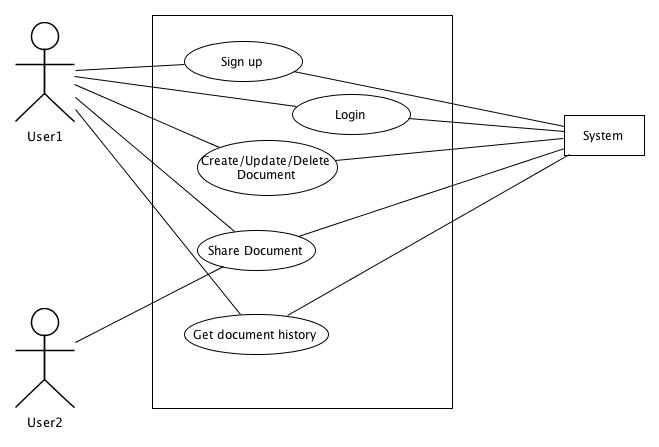
\includegraphics[width=300px]{images/UpdatedUsecaseDiagram.jpg}
    	\caption{Use-case diagram}
	\end{figure}
\subsection{Supplementary Specification (FURPS+)}
\label{sec-2-2}
Supplementary specification, along with use cases, show all the requirements that our system must fulfill.

\begin{itemize}
\item Functionality
\begin{itemize}
\item The system must be able to create/edit/delete users.
\item The system must be able to create/edit/delete/share documents.
\item The system must keep a log of all document actions.
\item All system usage requires user authentication.
\item The system must support multiple users.
\end{itemize}
\item Usability
\begin{itemize}
\item The system must be easy to use.
\begin{itemize}
\item Have a clean user interface.
\item 8 out of 10 users must be able to use the system without any training.
\end{itemize}
\item The system must be easily visible for people with ``not perfect'' vision. 
       E.g no graphics that blurs the view of the core system functionality.
\item The web client must be easy and quick to navigate. No function should 
       be more than 3 clicks (windows/sub-windows) away.
\begin{itemize}
\item Not counting navigating a users files.
\end{itemize}
\end{itemize}
\item Reliability
\begin{itemize}
\item It must be possible to use the system without any internet connection.
\begin{itemize}
\item With some limitations.
\end{itemize}
\end{itemize}
\item Performance
\begin{itemize}
\item The system must respond instantly
\begin{itemize}
\item A request must not take more than a few (2-3) seconds.
\item Not taking external factors (such as bad internet connection) into account.
\end{itemize}
\end{itemize}
\end{itemize}
\subsection{Domain Model}
\label{sec-2-3}
\begin{figure}[H]
  		\centering
    	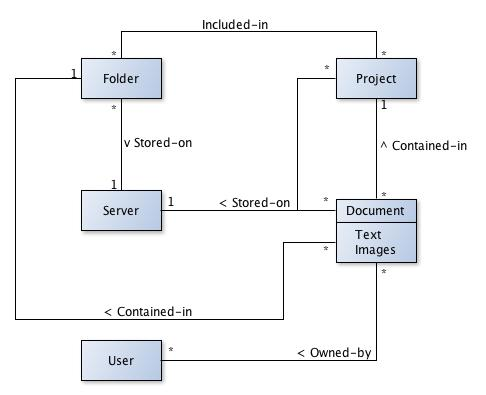
\includegraphics[width=300px]{images/DomainModel.jpg}
    	\caption{Domain Model}
\end{figure}
\subsection{Logical Architecture}
\label{sec-2-4}

   The logical architecture diagram shows a rough sketch off how the structure of the application
   will be like. This is by no means a complete diagram, but should give an idea off how
   the application will look like.
\begin{figure}[H]
  		\centering
    	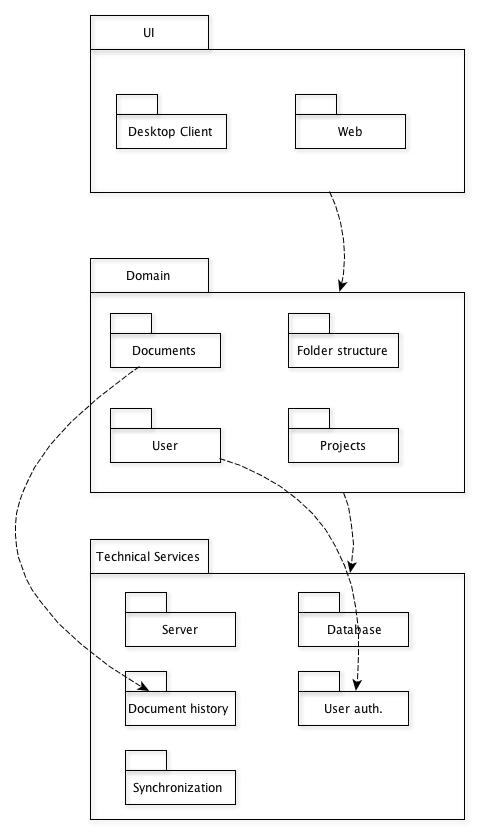
\includegraphics[width=300px]{images/LogicalArchitecture.jpg}
    	\caption{Logical Architecture}
\end{figure}
\subsection{System Sequence Diagram}
\label{sec-2-5}

   The diagram shows all the operations that are available to a regular user.
\begin{figure}[H]
  		\centering
    	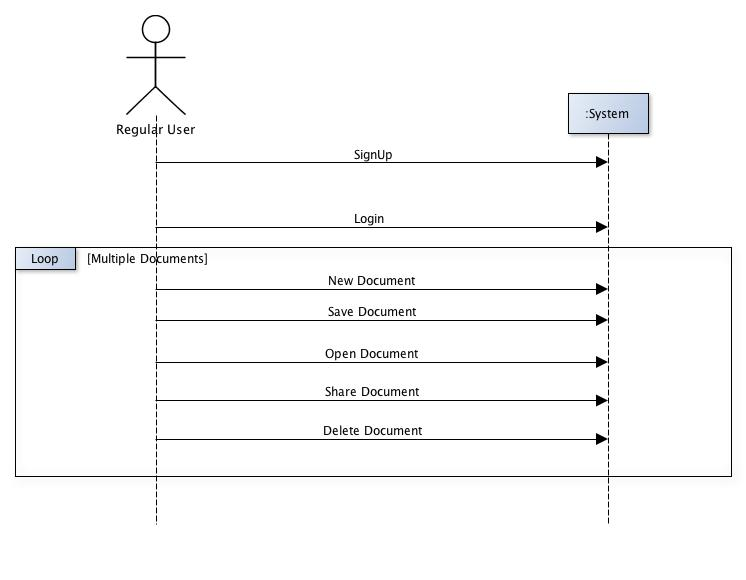
\includegraphics[width=300px]{images/Complete_SSQ.jpg}
    	\caption{System Sequence Diagram}
\end{figure}
\subsection{Operation Contracts}
\label{sec-2-6}

\fbox{\begin{minipage}{\columnwidth}
		\textbf{Contract CO1:} Synchronize / Merge \\
		\textbf{Operation:} Synchronize / Merge \\
		\textbf{Cross References:} UC1, UC2, UC4, UC5 \\
		\textbf{Preconditions:} Some documents and/or folders must have been created on the system. \\
		\textbf{Postconditions:} \\
		\begin{itemize}
		\item All documents and folders on the client must be uploaded to the server.
		\item All documents and folders on the server must be downloaded to the client.
		\item Document version must be the same on the client and server.
		\end{itemize}
\end{minipage}}

\section{Design}
\label{sec-3}
\subsection{Class Diagram}
\label{sec-3-1}
The class diagram show how our server side classes are connected. For a complete class diagram for all classes, along with methods and fields, see the \emph{appendix.}
\begin{figure}[H]
  		\centering
    	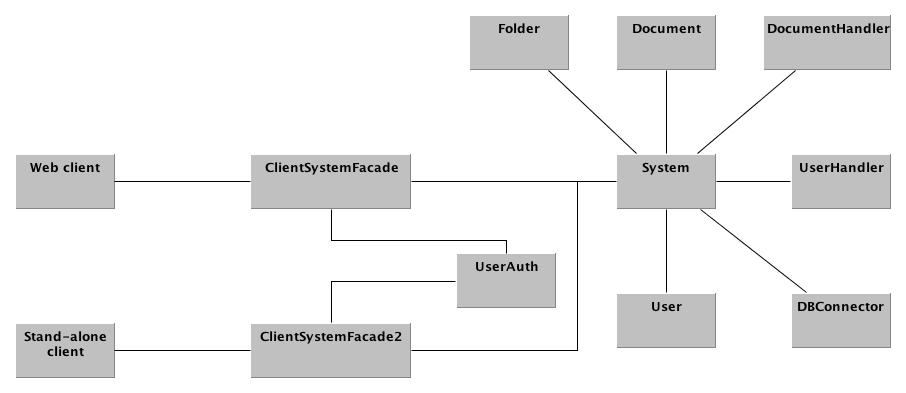
\includegraphics[width=300px]{images/LatestClassDiagram.jpg}
    	\caption{Class Diagram}
\end{figure}
\subsection{Interaction Diagrams}
\label{sec-3-2}
\subsubsection{Sequence Diagram}
\label{sec-3-2-1}
The SaveDocument() Sequence Diagram shows how the system communicates internally when the SaveDocument() method is called.
For other related methods (OpenDocument() ShareDocument() etc.. ) the program flow is the same (though they vary on some parameters and other details).
\begin{figure}[H]
  		\centering
    	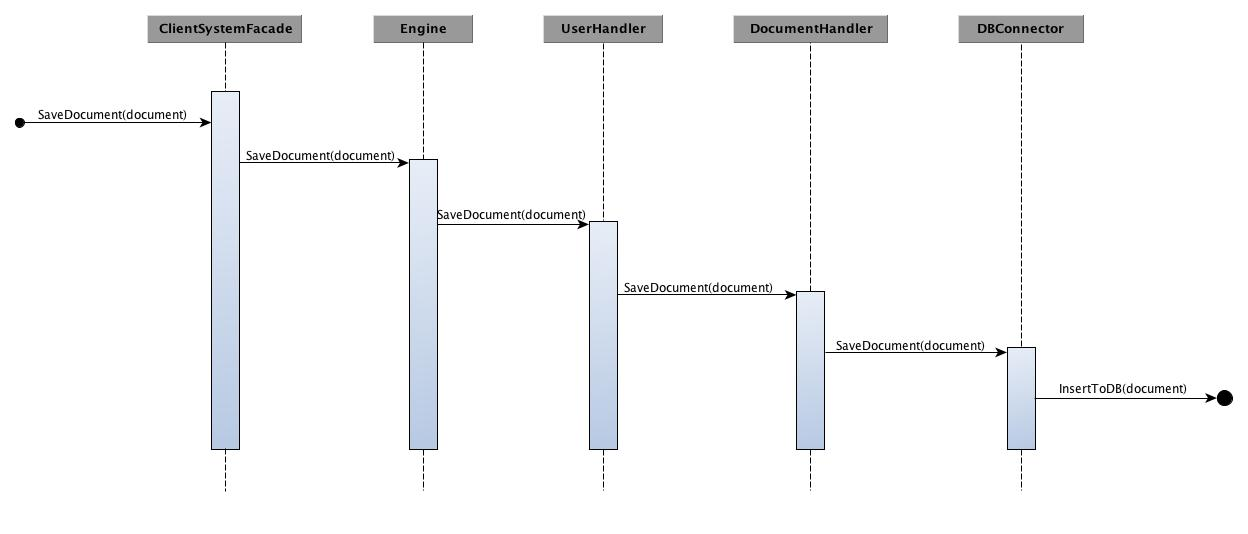
\includegraphics[width=300px]{images/SequenceDiagram_SaveDocument.jpg}
    	\caption{Sequence Diagram}
\end{figure}

\subsubsection{Communication Diagram}
\label{sec-3-2-2}
\begin{figure}[H]
  		\centering
    	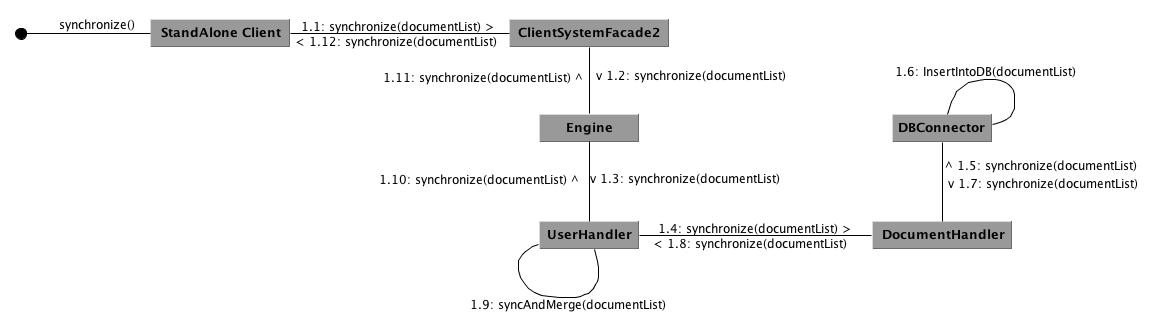
\includegraphics[width=300px]{images/CommunicationDiagram_Synchronize.jpg}
    	\caption{Communication Diagram}
\end{figure}

\subsection{ER-Diagram}
\label{sec-3-3}
\begin{figure}[H]
  		\centering
    	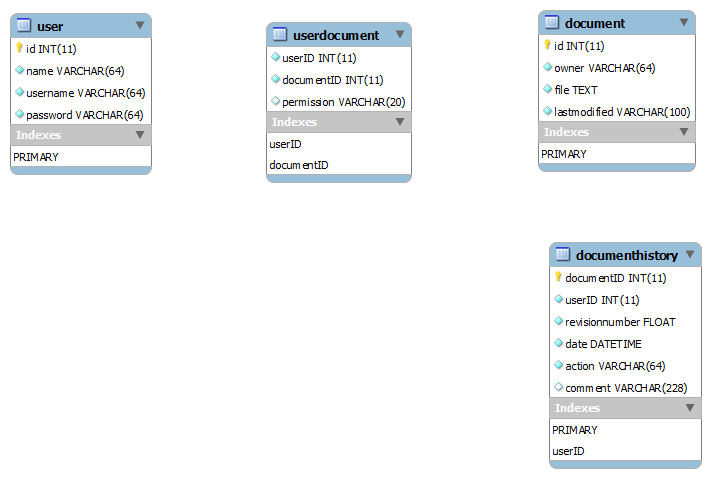
\includegraphics[width=300px]{images/New ER database.png}
    	\caption{ER-Diagram}
\end{figure}
\subsection{User manual}
\label{sec-3-4}
\subsubsection{Starting the application}
\label{sec-3-4-1}
\begin{itemize}

\item Running the application from Visual Studio\\
\label{sec-3-4-1-1}%
Before starting the application, you need to start Visual Studio with administration privileges.
The reason for this is that the application will need to create files and folders for the documents and in order to do so the program needs to be run with administrator privileges which will give the application write access.

Since the web client runs in the browser, the browser needs to allow pop up windows for localhost.
This can be done when the application is run for the first time.

When starting the application, you need to set the WebClient project as startup project (if it's not already set), and then run the program (f5 for debug mode, ctrl + f5 for the release version).

The web client will start up with your default internet browser. 
When the main page has loaded, you are ready to use the application.

\item Signing up\\
\label{sec-3-4-1-2}%
As a first time user there won't be any user registered in the system, so the first time you need to sign up to use the system.

To sign up, click the "Sign up'' button. This will open up a new window with the sign up form.

Fill out the form and click the "Sign up'' button. A message will appear to say if the sign up was successful or not.

If the sign up was successful you are now registered in the system, and are ready to use it. 
Close the sign up window and go back to the main window.

\item Logging in\\
\label{sec-3-4-1-3}%
On the main screen there are two text boxes at the top of the window named "username'' and "password''.
Enter the newly created username and password into the boxes and click the "Login'' button.
\end{itemize} % ends low level
\subsubsection{Using the Application}
\label{sec-3-4-2}

After you have logged in, press the "Get Files'' button on the left page of the window. 
This will show you all the files that belong to the current user. Since you are a new user you don't have any documents, so you should only see the root folder (the one with your username).
\begin{itemize}

\item Create a new document.\\
\label{sec-3-4-2-1}%
To create a new document, click the "New Document''. This will clear all text boxes, and you are ready to write a new document.

Creating a new document doesn't save the document, so before you go too far you should save your document.
Write a file name in the file name box, and click the ``Save Document'' button.
If you wish to save the document in a sub folder, just write: "folder name/file name.html'' in the file box.

The system doesn't require that you save the document as a HTML file, but the system is built around it. Not doing so won't make it able to add images to you document.

\item Deleting a document\\
\label{sec-3-4-2-2}%
Deleting a document is very simple.
Select a document from the list on the left. Make sure that the filename of the file is entered into the file name box (this can also be done manually). Delete the document by clicking the "Delete Document'' button.

\item Sharing a document\\
\label{sec-3-4-2-3}%
Sharing a document is very simple as well.
Open the document you wish to share. Enter the user name of the user you wish to share the document with in the text box next to the "Share Document'' button, and click the share document button.

\item Showing a document\\
\label{sec-3-4-2-4}%
Since the document is built around the HTML format, the text area can't show any images or text formatting.
In order to see the document (with images, formatting etc) you need to open it in another page in the browser.
Select the document you wish to view and click the "Show Document'' button. This will open a new window with your document in parsed HTML.

\end{itemize} % ends low level
\section{Implementation}
\label{sec-4}
\subsection{Software Architecture Document}
\label{sec-4-1}
\subsubsection{Architectural Representation}
\label{sec-4-1-1}

The SAD summarizes the architecture of the Slice of Pie application from multiple views. These views include:
\begin{itemize}
\item Logical view
\item Deployment view
\item Process view
\item Data view
\item Use-case view
\end{itemize}
\subsubsection{Architectural Factors}
\label{sec-4-1-2}

\begin{itemize}
\item Supplementary specifications.
\end{itemize}
\subsubsection{Architectural Decisions}
\label{sec-4-1-3}
\begin{itemize}
\item Technical Memos

\label{sec-4-1-3-1}%
\fbox{\begin{minipage}{\columnwidth}
\textbf{Issue:} Files format - Which file format to use \\
\textbf{Solution Summary:} Use HTML for our file format. \\
\textbf{Factors:}
\begin{itemize}
\item Must be able to contain both text and images.
\end{itemize}
\textbf{Solution:}
We chose to use HTML for our file format because it's simple to construct, and can contain text and images seamlessly. \\
\textbf{Motivation:} \\
We needed a file format that can contain images and text as well as being easy to construct. in addition, HTML can easily be extended to other content. \\
Lastly, HTML can be opened with any browser, so the users isn't tied to SliceOfPie if he just want's to view the content of a file. \\
\textbf{Alternatives considered:} \\
We considered using a .txt file format, but .txt can only contain plain text.
We also considered using our own file format (since the format itself isn't important to the application). But if we use our own format the user is stuck
with using SliceOfPie, so he can't view the content of a file with any other application.
\end{minipage}}

\fbox{\begin{minipage}{\columnwidth}
\textbf{Issue:} Merging two versions of the same document. \\
\textbf{Solution Summary:} Git-hub inspired merge. \\
\textbf{Factors:}
\begin{itemize}
\item Merging two versions of the same document without overwriting existing changes.
\end{itemize}
\textbf{Solution:}
Our merging algorithm reads the two documents and stores them, line by line in an array. 
Then the algorithm compares each line in the two arrays, if the lines are the same, insert the line into a new array. If the two lines aren't identical, insert the new line into the new array + insert the line from the old array in the next line. This line will be encapsulated with $<<<$ TEXT $>>>$ which shows the user where there is a conflict which the user can solve later on. 
If the new version of the document contains lines that aren't in the old array, they are simply added to the new array. 
\textbf{Motivation:} \\
There are other, more advanced, merging algorithms available. Because of time constraint we chose to use this one. It isn't the most advanced/complete algorithm but it does the job quite well considered it's simplicity. \\
\textbf{Unresolved issues:} \\
\begin{itemize}
\item Our algorithm doesn't 100\% solve the conflict. In the end the user must manually chose which version to keep, and which version to discard.
\item If two identical lines exists in both versions but the lines is at another line number in the old document, this might cause a conflict $<<<$ TEXT $>>$ that could be avoided.
\end{itemize}
\textbf{Alternatives considered:} \\
An algorithm that analyses every line in the file keeps the one that the user wants.
\end{minipage}}

\fbox{\begin{minipage}{\columnwidth}
\textbf{Issue:} Choosing how to connect to the database \\
\textbf{Solution Summary:} Simplest option due to time pressure \\
\textbf{Factors:}
\begin{itemize}
\item Simplicity
\item Easy to get working
\end{itemize}
\textbf{Solution:} \\
Our way of connecting to the database, and executing queries on it is a series of methods close to hard coded SQL queries. they do not automatically update if a table/column/attribute were to change. \\
\textbf{Motivation:} \\
Early in the process we also designed a solid design for the database, which meant that we were able to make the "final'' outcast of the database rather quickly. \\
And looking apart from the fact that the solution does not adapt to changes made on the database, it works perfectly and required minimal attention and time to get working. \\
\textbf{Alternatives considered:} \\
Entity framework was a possibility from the start, but since entity framework had proven a challenge to get working for all of us in the past, we choose the, for us at the time, simpler solution to save time in the end
\end{minipage}}

\end{itemize} % ends low level

\subsubsection{Logical View}
\label{sec-4-1-4}

\begin{itemize}
\item Logical diagrams etc ..
\end{itemize}
\subsubsection{Deployment View}
\label{sec-4-1-5}

\begin{itemize}
\item Delpoyment diagrams etc \ldots{}
\end{itemize}
\subsubsection{Process View}
\label{sec-4-1-6}

\begin{itemize}
\item Interction diagrams etc ..
\item Class diagrams
\end{itemize}

    Comment on how the inter process communication works.
\subsubsection{Use-Case View}
\label{sec-4-1-7}

\begin{itemize}
\item Use cases
\item Use case diagrams
\end{itemize}
\subsubsection{Other Views \ldots{}}
\label{sec-4-1-8}
\section{Project Management}
\label{sec-5}
\subsection{SCRUM}
\label{sec-5-1}
\subsubsection{Definition of done}
\label{sec-5-1-1}

Before our system is ready for release, we must have implemented all required features.
In addition to implementing the features, we also must document every aspect of the system
and the process. This includes diagrams, use cases etc \ldots{}
Finally we have to test our system to make sure that it works as intended and doesn't break 
when receiving odd input etc..

A more detailed explanation of the requirements can be found below.
\begin{itemize}

\item Development\\
\label{sec-5-1-1-1}%
The system must be able to handle all the requirements before it can be deemed done.
These requirements include the assignment required requirements as well as our
own requirements.

These requirements include:
\begin{itemize}
\item $\boxminus$ Document [3/4]
\begin{itemize}
\item $\boxtimes$ Create a document that can handle both text and images.
\item $\boxtimes$ Documents can be arranged into folders.
\item $\Box$ Documents can be arranged into projects (optional).
\item $\boxtimes$ Log of all changes to a document.
\end{itemize}
\item $\boxtimes$ System [4/4]
\begin{itemize}
\item $\boxtimes$ Synchronization for offline usage.
\item $\boxtimes$ Sharing of documents to other users.
\item $\boxtimes$ Authentication system for users.
\item $\boxtimes$ Document storage in a database.
\end{itemize}
\item $\boxtimes$ User Interface [2/2]
\begin{itemize}
\item $\boxtimes$ Web interface.
\item $\boxtimes$ Stand-alone client (for offline usage).
\end{itemize}
\end{itemize}


\item Documentation\\
\label{sec-5-1-1-2}%
All aspects of the system must be documented.
The idea of the documentation is that the system is easy to understand based only on
the documentation. In addition, an external actor must be able to see the development
process from reading the documentation only.

These documents must be made before the documentation can be deemed as done:
\begin{itemize}
\item $\boxtimes$ Use cases [3/3]
\begin{itemize}
\item $\boxtimes$ All use cases must be documented (text form)
\item $\boxtimes$ Use case diagram must be made for use cases that require it.
\item $\boxtimes$ Operation contracts must be made for use cases that are complex.
\end{itemize}
\item $\boxtimes$ Domain documentation [2/2]
\begin{itemize}
\item $\boxtimes$ A model must be made for describing the domain.
\item $\boxtimes$ A sequence diagram must be made for understanding how to domain
       interacts.
\end{itemize}
\item $\boxtimes$ Software documentation [4/4]
\begin{itemize}
\item $\boxtimes$ Static class diagram that explains the entire system.
\item $\boxtimes$ Package diagram that shows a higher view of the system.
\item $\boxtimes$ Interaction diagrams that describe the dynamic aspect of the system.
\item $\boxtimes$ E-R diagram for the database structure.
\end{itemize}
\end{itemize}


\item Testing\\
\label{sec-5-1-1-3}%
Before the system can be declared done, all the core features of the system
must be thoroughly tested.
This includes testing all core features of the system.

Testing checklist:
\begin{itemize}
\item $\Box$ System [0/8]
\begin{itemize}
\item $\Box$ Document
\item $\Box$ DocumentHandler
\item $\Box$ Folder
\item $\Box$ User
\item $\Box$ UserAuth
\item $\Box$ DBConnector
\item $\Box$ ClientSystemFacade
\item $\Box$ ServerSystemFacade
\end{itemize}
\item $\Box$ Client [0/2]
\begin{itemize}
\item $\Box$ Stand-Alone client
\item $\Box$ Web-Client
\end{itemize}
\end{itemize}

\end{itemize} % ends low level
\subsubsection{Product Backlog}
\label{sec-5-1-2}
\subsubsection{Intro}
\label{sec-5-1-3}
\subsubsection{Sprints}
\label{sec-5-1-4}
\begin{itemize}

\item 1. sprint
\label{sec-5-1-4-1}%
\begin{itemize}
\item Sprint backlog
\item Burndown chart
       \textbf{Review:}
\begin{itemize}
\item Items were completed easier than first anticipated
\item To few items in sprint
\item Basic understanding of systems functionality is now documented in form of use cases
\end{itemize}
\textbf{Retrospective:}
\begin{itemize}
\item Group works together great
\item Private lives (jobs, other classes, sports, etc.) interfeering with most available
         ``Work-days'', group members are trying to postpone future non-project related activities
\end{itemize}
\end{itemize}

\item 2. sprint
\label{sec-5-1-4-2}%
\begin{itemize}
\item Sprint backlog
\item Burndown chart
\end{itemize}
     \textbf{Review:}
\begin{itemize}
\item Items were easier compleeted tha first anticipated
\item To few items in sprint
\item Started coding for real
\item Basic system arctitecture taking form
\end{itemize}
     \textbf{Retrospective:}
\begin{itemize}
\item Members finishing their private arrangements (jobs, other classes, sports, etc.)
       Getting more time from next sprint on
\end{itemize}

\item 3. sprint
\label{sec-5-1-4-3}%
\begin{itemize}
\item Sprint backlog
\item Burndown chart
\end{itemize}
     \textbf{Review:}
\begin{itemize}
\item Items took longer than expected to comlpete
\item Finished building seperate code, started to implement main features using eachother
       instead of test data, encountered more errors than expected and will take alot of
       work to fix
\end{itemize}

     \textbf{Retrospective:}
\begin{itemize}
\item Members had most time free to work on project, but due to unexpected errors
       sprint was not successfully finished
\item Memebrs still working great together, despite the pressure
\end{itemize}


\item Chaos sprint\\
\label{sec-5-1-4-4}%
\textbf{Review:}
\begin{itemize}
\item Most optional functionality were not implemented due to the lack of time
\item All required functionality completed, though with small ``bugs/features''
\end{itemize}

     \textbf{Retrospective:}
\begin{itemize}
\item Members used all spare time they had on the project, but had to drop
       alot of ``optional work'' to get the program done.
\item Writing the report happened to late acording to plan (due to the program
       not being done), but scrum has been followed up un every ``work-day''
       which made the report-writing quite easier.
\end{itemize}
\end{itemize} % ends low level
\subsubsection{Review}
\label{sec-5-1-5}

    The last sprint was chaotic for the members, since their last normal sprint 
    took longer than expected, due to this no sprint backlog was created since 
    most work was getting individually coded function to cooperate.
    Had it not been for a slow start the team would have had a more descriptive
    finishing sprint, and a more linear release burndown chart.
    
    Most of this is caused by the number of members in the team/group, and their 
    experience in being a ``SCRUM-Master'', since there were only 3 members, 
    there was not capacity for only one of the members to be SCRUM-Master.
    
    And without one single SCRUM-Master it was hard for the group to calculate
    the efford of each backlog item. Most of the Team's problems could have been
    solved by better planning more in the beginning of the project, and more time set 
    aside for the actual planning of each sprint.
    
    Private lives also interfered in the project, and this could be avoided by each
    member planning more carefully what they need to do in the project time period 
    

\end{document}
